\chapter{Drools}

Zur Realisierung des Workflow-Mechanismus wird die Rule Engine Drools\footnote{siehe auch http://www.drools.org} verwendet.\par
Daf�r wird eine Regelbasis in XML f�r drool erzeugt, die im Wesentlichen aus Regeln besteht, die sich in drei Teile gliedern lassen: Parameter, Bedingung und Konsequenz. Diese Regelbasis wird sich auf dem Server befinden. \par
Wenn ein Client eine Aktion dem Server meldet, so wird dieses Ereignis auf die Regelbasis angewendet. Es werden dabei alle Regeln durchlaufen. Stimmt das Ereignis mit der Bedingung einer Regel �berein, so wird die Konsequenz dieser ausgef�hrt. Die Ergebnisse dieser Regelkonsequenzen werden zu einem Workflow-Objekt zusammengef�gt (zum Beispiel eine Reihe von Anweisungen). Diese Workflow-Objekt wird dann auf die Message-Queues der Clients gelegt, f�r die das Workflow-Objekt relevant ist. Beim n�chsten Login des Clients, wird diese Objekt dann gepollt und in die Workflow-View des Benutzers gef�gt.\newline
\newline
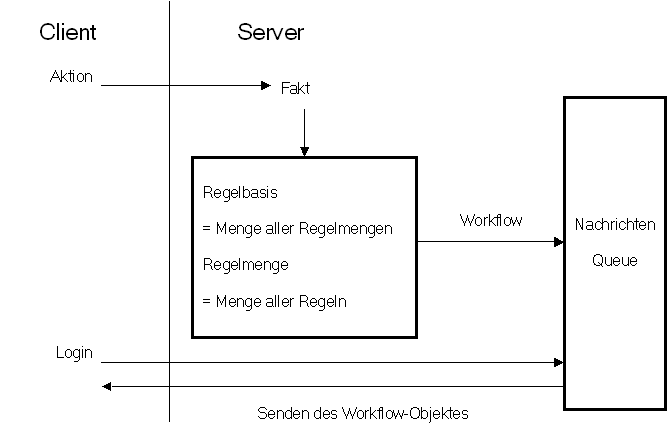
\includegraphics[width=15cm]{drools.png}\newline
Ein Workflow-Objekt ist dabei eine Art XML-Struktur, die einen Titel und eine Liste aller Regelresultate besitzt.\par
Kobold wird eine Anfangsregelbasis zur Verf�gung stellen, die vom Anwender jederzeit erweitert werden kann. Daf�r muss dieser nur eine neue Regel erstellen. Daf�r wird ihm ein Editor zur Verf�gung stehen, der in einer der kommenden Iterationen entstehen wird. Diese Regeln m�ssen dann nicht unbedingt zum Workflow-Objekt hinzugef�gt werden sondern k�nnen in ihrem Konsequenzteil auch andere Aktionen ausf�hren. Dies bleibt dem Anwender �berlassen.